\documentclass{article}
\usepackage{graphicx}
\graphicspath{{./images/}}
\usepackage{geometry}
\usepackage{hyperref}
\usepackage{paralist}
\usepackage[round]{natbib}
\usepackage{sectsty}
\usepackage{gensymb}
\usepackage{caption}
\usepackage{subcaption}
\usepackage{listings}
\usepackage[space]{grffile}
\usepackage{latexsym}
\usepackage{amsfonts,amsmath,amssymb}
\usepackage{url}
\usepackage{hyperref}
\hypersetup{colorlinks=false,pdfborder={0 0 0}}
\usepackage{textcomp}
\usepackage{longtable}
\usepackage{multirow,booktabs}
\newcommand{\truncateit}[1]{\truncate{0.8\textwidth}{#1}}
\newcommand{\scititle}[1]{\title[\truncateit{#1}]{#1}} 
\usepackage[parfill]{parskip}
\usepackage[final]{pdfpages}

% Typeface
\usepackage{ifxetex}
\ifxetex
  \usepackage{fontspec}
  \defaultfontfeatures{Ligatures=TeX} % To support LaTeX quoting style
  \setmainfont[Mapping=tex-text, Color=textcolor]{HelveticaNeue}
\else
  \usepackage[T1]{fontenc}
  \usepackage[utf8]{inputenc}
  \renewcommand{\familydefault}{\sfdefault}
  \usepackage{helvet}
\fi
\chapterfont{\Large} % \sffamily

% Title page
\usepackage{xcolor}
\definecolor{titlepagecolor}{cmyk}{0,0,0,0}
\definecolor{namecolor}{cmyk}{0,0,0,1} 
\definecolor{chaptertitlepagecolor}{cmyk}{0,0,0,0.9}
\definecolor{chapternamecolor}{cmyk}{0,0,0,0.3}  

\begin{document}

% ---------------------------------------------- TITLE PAGE ----------------------------------------------
\begin{titlepage}
\newgeometry{left=7.5cm} %defines the geometry for the titlepage
\pagecolor{titlepagecolor}
\noindent
%\includegraphics[width=2cm]{images/sage.pdf}\\[-1em]
%\includegraphics[width=2cm]{images/sage.png}\\[-1em]
\color{black}
\textbf{\textsf{Brendan Alexander Harmon}}\\
\makebox[0pt][l]{\rule{1.3\textwidth}{1pt}}
\par
\noindent
%\textbf{\textsf{North Carolina State University}} \textcolor{namecolor}{\textsf{PhD in Design}}
%\textbf{\textsf{Brendan Alexander Harmon}} 
\textcolor{namecolor}{\textsf{North Carolina State University}}
\vfill
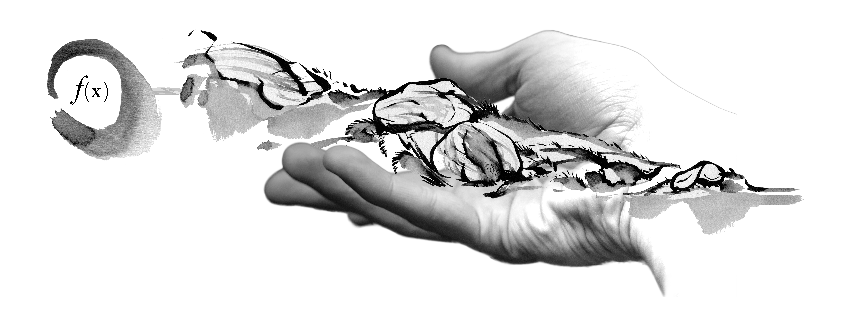
\includegraphics{images/tangible_landscape_diagram.pdf}
%\includegraphics[width=\textwidth]{images/procedural_landscape.png}
\vfill
\noindent
{\huge \textsf{Tangible Landscape}}
\vskip\baselineskip
\noindent
\textsf{October 2015}
\end{titlepage}
\restoregeometry % restores the geometry
\pagecolor{white}

\end{document}

